\chapter{Speech Recognition and Analysis Methods}
\label{ASR}

In this section, we will turn from the scientific investigation of spoken language and the research tools that are currently used for this purpose to the engineering side of recent developments. We will first contemplate on the astonishing rise of the field of automated speech recognition, and then discuss in some detail current software instruments that were developed to aid this purpose. This is meant as a survey with the intention to select the tools that could be used to achieve the goal to assist scientific research in individual spoken languages.

\section{Automated speech recognition}

Automated speech recognition (ASR) is now ubiquitous: voice assistants, call centers, subtitle generation, and multilingual conversation are commonplace. This capability required decades of sustained research to achieve. In fact, the importance of automatically transferring speech to a symbolic representation of language was identified right with the advent of digital computers. In 1952, Bell Labs built a recognizer that identified single digits spoken by a particular speaker from the vowel formants \cite{juang2005}. By the 1980's, the first automated typewriting machines became available and trained to individual speakers. In the early 2000's, ASR began to handle large vocabularies across multiple languages and independently of particular speakers, and it is increasingly used to identify speakers and their current emotional states.

Several technological and conceptual breakthroughs were made \cite{juang2005}. One important shift around 1980 was from pattern-recognition templates to Hidden Markov Models, with statistically motivated expectations about the following units based on preceding units. The stochastic nature of HMMs was able to cope with the high variability of spoken language between speakers and between speakers. HMMs were combined with finite-state networks to enable the identification of words and phrases. There was one problem: HMMs connect static frames, but these frames lack the uniformity of symbolic representations due to the high variability of speech data. This was solved using Gaussian mixture models that assess how well each HMM state fits a frame or a short window of frames. The next breakthrough came in the early 2000's with deep neural networks. The technology of neural networks, itself going back to the 1950's, had already been applied around 1990, but the emerging technology of deep neural networks with many hidden layers could achieve much better results \cite{hinton2012}. This allowed extensive pre-training of networks on a wide variety of inputs, essentially the same technique used in image recognition. Newer developments feature a more general transformation of acoustic features into word and phrase chunks that avoids the phoneme level \cite{chan2015}, and the combination of convolutional neural networks and transformers to model both local and global dependencies \cite{gulati2020}. Notice that these latter developments occurred within large companies like Microsoft, Google, and Amazon.

The massive technological development driven by the enormous potential economic benefit of speech recognition has led to a number of tools that are crucial for our own task, the automatic recognition of segmental and prosodic features across speakers and languages. We will turn to such tools in the following section.

\section{Phoneme and prosody recognizers}

We organize this section by first looking at speech recognizers that aim to convert spoken language into orthographically represented language, typically in the language's standard orthography. We then turn to tools that also identify the timing of the words and the individual phonemes. Finally, we will discuss tools that determine, in addition to segmental features, prosodic features such as pitch and amplitude.

\subsection{Speech recognizer: wav2vec, HuBERT, Whisper}

The tools to be surveyed here, wav2vec 2.0 \cite{baevski2020} and HuBERT \cite{hsu2021hubert}, are self-supervised speech encoders that learn from unlabeled audio or coarsely labeled speech clusters, with particular utility for low-resource languages. Both are designed to be fine-tuned for downstream ASR tasks.

Whisper \cite{radford2023whisper} used weak supervision on a large internet audio corpus (680,000 hours) with imperfect transcripts, captions, and translations. Unlike self-supervised approaches, the scale and diversity of training data enabled strong zero-shot generalization without dataset-specific fine-tuning. It operates as a sequence-to-sequence transformer, accepting audio and producing text tokens end-to-end.

Whisper natively supports 99 languages, though its performance varies significantly with the volume of training data; for instance, 65\% of its 680,000-hour pre-training corpus was English. This leads to high robustness for high-resource languages but creates a performance gap for low-resource languages, which often require fine-tuning to reach usable accuracy levels. Because the model's byte-pair encoding (BPE) tokenizer is fixed during pre-training, adding a truly new language for which no token exists (e.g., specific endangered dialects) is technically challenging. Researchers can bypass this by forcing the model to use an existing language code as a proxy. While Whisper excels at orthographic transcription and timestamp prediction for subtitles, it does not natively produce phonetic output in the International Phonetic Alphabet (IPA). For the purpose of precise phonetic and prosodic research, Whisper must be integrated into a broader pipeline.

The tool WhisperX \cite{bain2023whisperx} is an extension built on top of Whisper to address certain limitations. It provides more accurate timing, especially word-level timestamps, and can also provide speaker labels for recordings with multiple speakers. Based on automatic speech recognition by Whisper, it includes a voice activity detection to identify when speech is present, splitting the audio into better chunks before transcription. This is important for recordings of conversation "in the wild" (as opposed to in a lab experiment), as they often contain background noise. Cutting and merging audio into roughly 30-second chunks makes longer audio easier to process. Forced phoneme alignment (see the next paragraph) aligns the transcript with the audio, producing more accurate world-level timestamps. Speaker diarization: optionally assigns speaker labels to different parts of the transcript.

% more about languages, kind of output, IPA?

\subsection{Phoneme aligners: Montreal Forced Aligner (MFA)}

The task of speech recognizers is to create, from spoken input, a written representation, typically using the standard orthography of a language or a narrower transcription, as in IPA. However, this does not provide information about the timing and realization of the phonemes corresponding to these graphemes in the speech signal. Such information about when phonemes and words are realized may be necessary to answer many research questions. For example, we might be interested in the distribution of pauses, the formation of prosodic phrases, the distinction between short and long syllables in languages that make this distinction, or slowing and speeding up related to the beginning or end of prosodic units. This is the task of phoneme aligners: they generally assume an orthographic transcription and provide information about the temporal alignment of these representations in the audio signal. This information can then be represented as annotation tiers in phonetic analysis programs such as Praat.

For example, Whisper includes a timestamp for utterances (typically an utterance surrounded by pauses), which is important, for example, for creating subtitles for video. To overcome the weaknesses of this component, \cite{bain2023whisperx} developed a tool, WhisperX, that significantly improves timing. The program extends timing to individual words and phonemes.

There are several programs on the market that perform a more precise time alignment of phonemes. For example, WebMAUS \cite{kisler2012} is being developed as a web-based service to generate time-aligned phonemes for recordings in languages that were pre-trained with hand-annotated phonemic transcriptions. In contrast, MFA, the Montreal Forced Aligner is a stand-alone tool that was pretrained on many languages. It was developed at McGill University \cite{mcauliffe2017mfa}. Additional documentation and downloads are available on the official website: \url{https://montreal-forced-aligner.readthedocs.io/en/latest/}. MFA is trained on a limited amount of data in several steps, first by attempting individual phoneme recognition, followed by trigram recognition, where a phoneme is identified in the context of surrounding phonemes, according to the phonological rules of a language. In the training phase, MFA performs 40 iterations. The MFA comes pre-trained for several languages.  The alignment performs well on the large LibriSpeech corpus for English. As of 2026, MFA has been trained on 50 languages, with several models for some of the larger languages. For languages not on the list it is recommended to use a phonologically similar language as a bootstrap and then train MFA on that language. The resulting timestamps are more accurate than those achieved by WhisperX, according to https://github.com/m-bain/whisperX/issues/1247.

\begin{figure}[htbp]
    \centering
    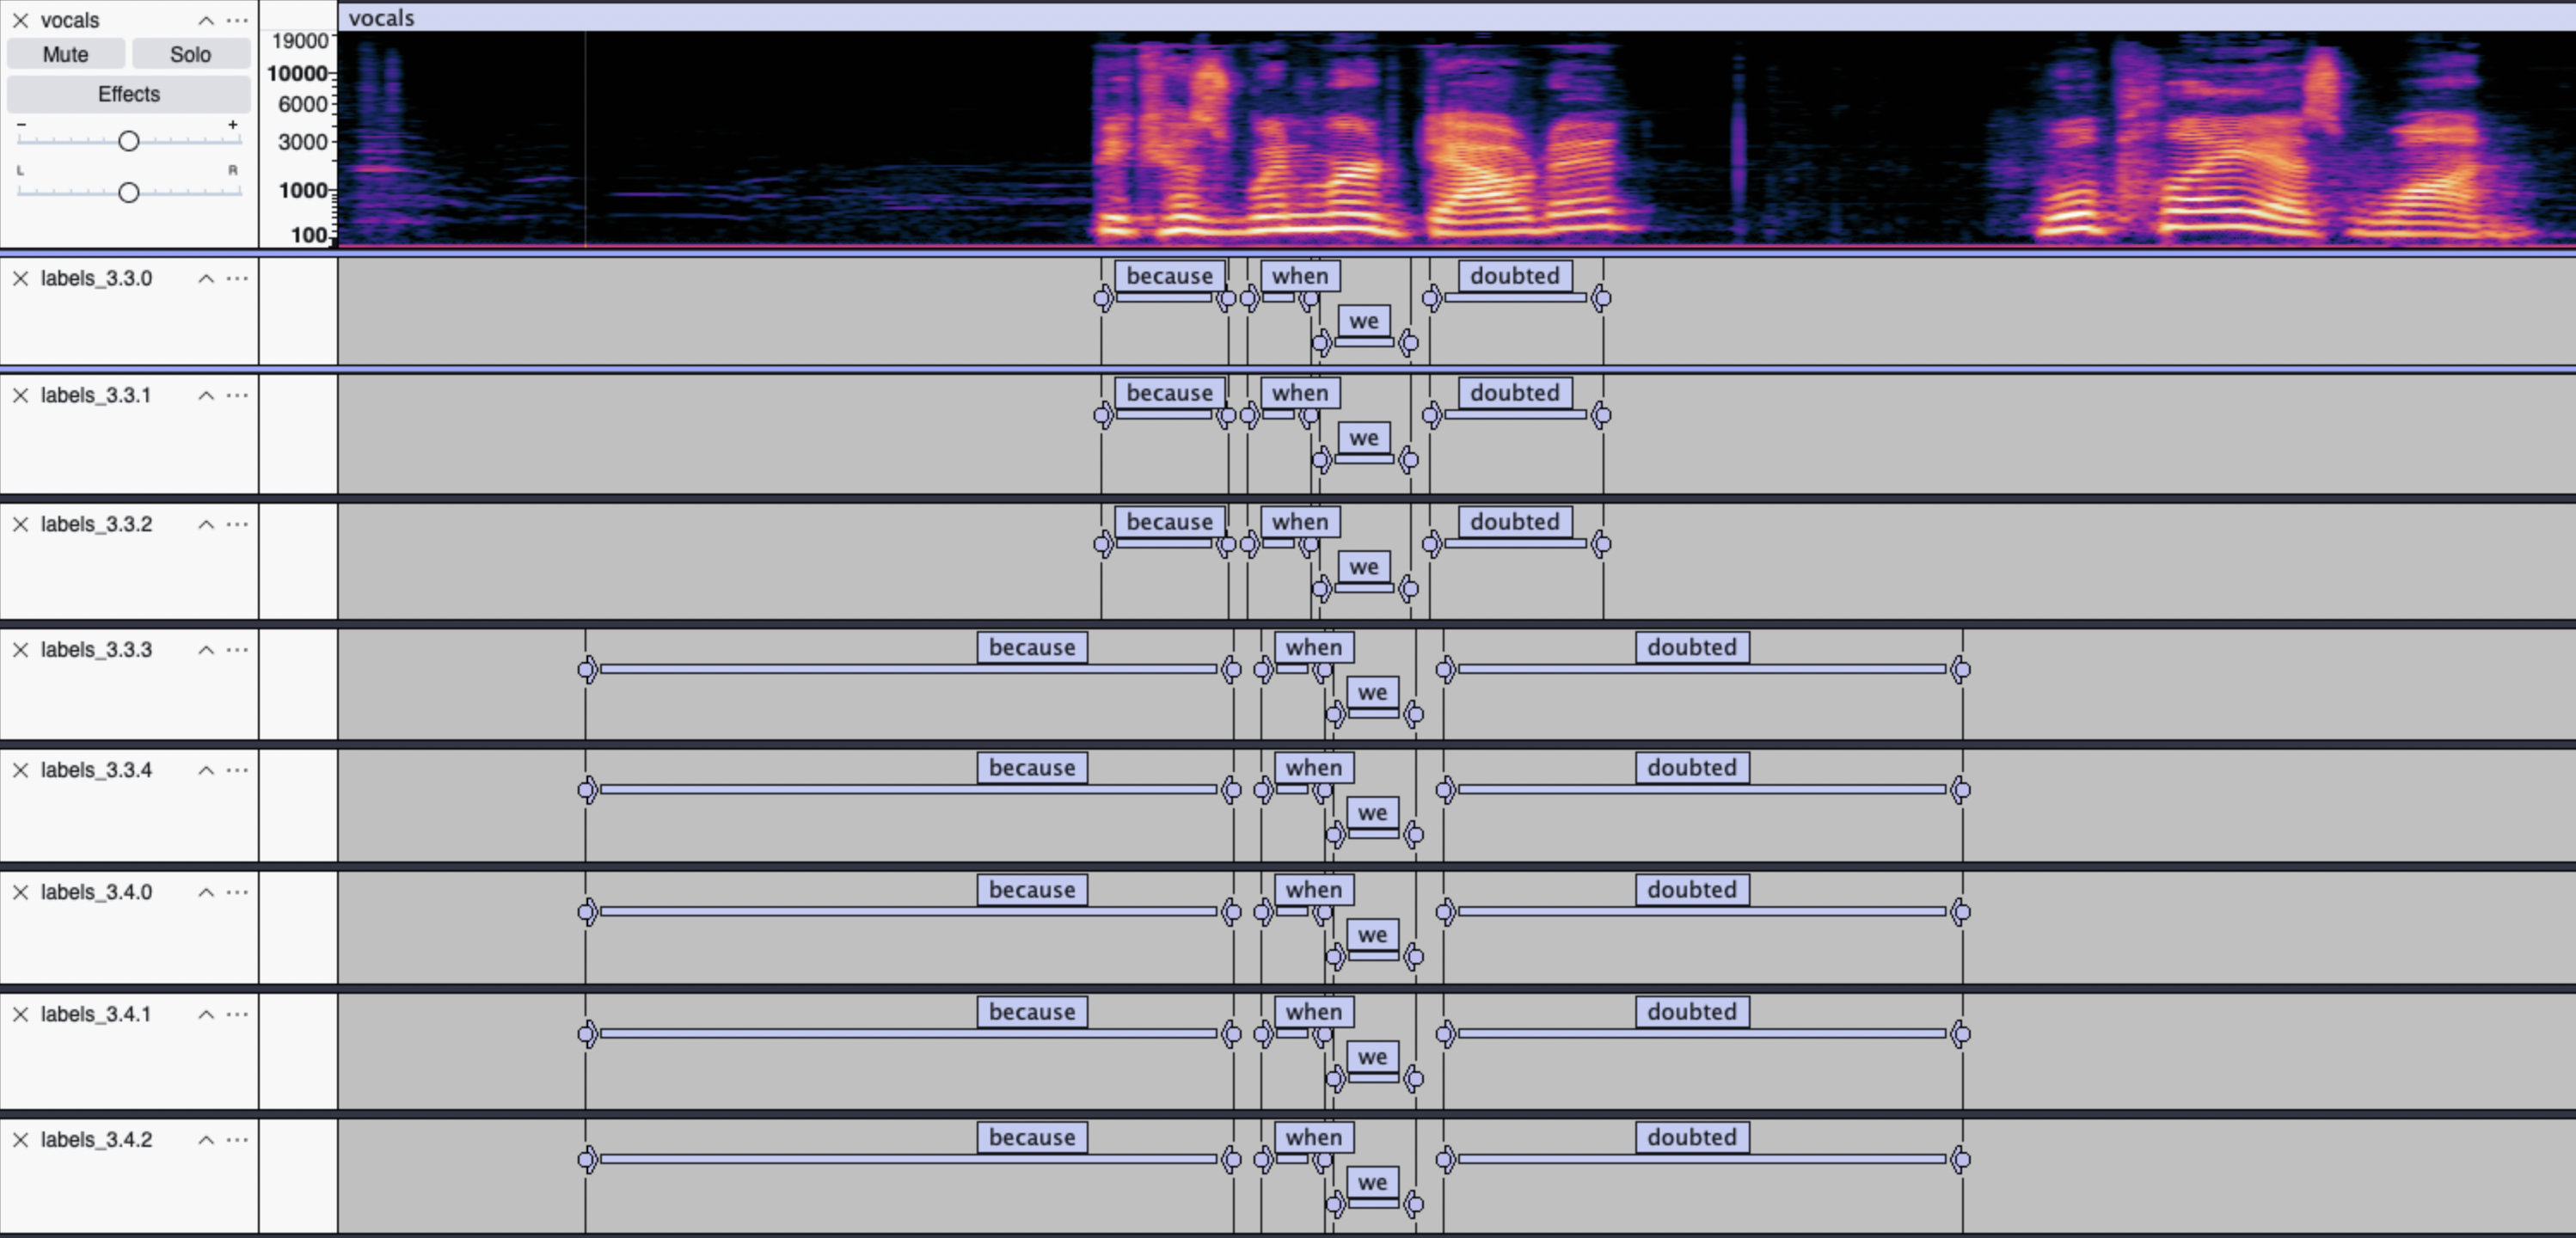
\includegraphics[width=\textwidth]{introduction/whisperx_regression_audacity.png}
    \caption{Comparative analysis in Audacity showing word-level timestamp drift in WhisperX versions 3.3.0 through 3.4.2. Note the lack of tight alignment with the audio signal following the version 3.3.3 regression \cite{bain2025whisperxissues1220}.}
    \label{fig:whisperx_drift}
\end{figure}

\begin{figure}[h]
    \centering
    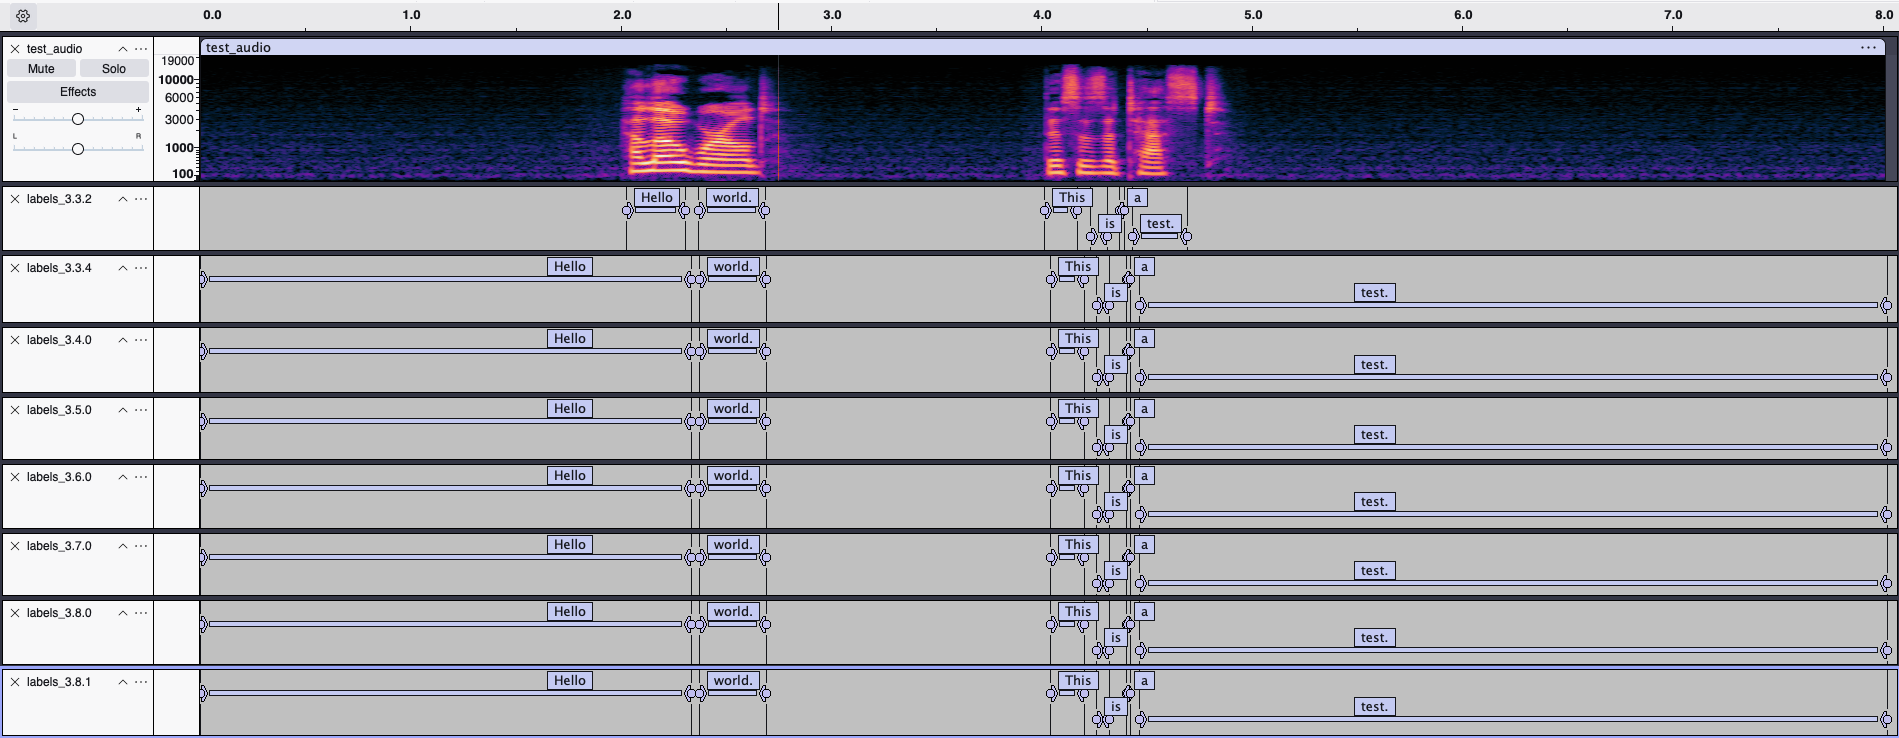
\includegraphics[width=0.92\linewidth]{introduction/whisperxfeb22.png}
    \caption{Persistent timestamp regressions in WhisperX versions up to 3.8.1. The issue concerns premature segment triggering and alignment instability motivating the comparative multi-aligner architecture adopted in \textit{SpeechPrint}.}
    \label{fig:whisperx_timestamp_issue}
\end{figure}

Applying a search on the Open ASR Leaderboard \cite{srivastav2025} (current as of May 24, 2026, via Hugging Face), we identified Whisper-Large-v3 (\url{https://whisper-v3.com/} as a frontrunner among the open-source tools when considering the average WER, or Word Error Rate of 2.77 \% and a high number of supported languages (99). It was trained on 1 million hours of diverse, weakly labeled audio and is robust against background noise and varied accents. It shows improved performance across a wide variety of languages, with a 10\% to 20\% reduction in errors compared to Whisper large-v2.

Despite the strong alignment quality of MFA, several practical engineering limitations influenced the final design decisions of \textit{SpeechPrint}. MFA is notoriously difficult to install and does not currently integrate naturally with lightweight \texttt{uv}-managed Python workflows used throughout this research. Furthermore, we observed that MFA crashes with files longer than approximately 10 seconds in duration, necessitating the audio to be processed in small chunks.

The initial design used \textbf{WhisperX} as the primary aligner. However, internal testing identified substantial timestamp accuracy regressions beginning with version 3.3.3 \cite{bain2025whisperxissues1220}, with errors up to 7.6s \cite{bain2025whisperxissues1220}. Because SpeechPrint requires millisecond-level accuracy for synchronized $F_0$ and amplitude extraction, these regressions necessitated a hybrid approach combining Whisper's transcription with more stable aligners (Gentle or MFA).


For this reason, \textit{SpeechPrint} ultimately adopts a hybrid pipeline combining Whisper, CrisperWhisper, and \textbf{Gentle} \cite{ochshorn2015gentle}. While WhisperX is utilized for its robust Voice Activity Detection (VAD) and batching capabilities, the framework relies on Gentle or MFA for the actual alignment. Gentle, a toolkit built on \textbf{Kaldi}, is integrated for its ``robust yet lenient'' behavior, which maintains stable long-form alignment even in the noisy field recordings typical of the \textbf{DoReCo} dataset. This design prioritizes reproducibility, maintainability, and compatibility with modern Python environments while ensuring sufficiently accurate temporal segmentation for prosodic feature extraction.

The resulting pipeline produces time-aligned TextGrid files with word, phoneme, and syllable layers, plus pitch and prosodic annotations, exported alongside CSV/JSON metadata for inspection and correction. For downstream analysis, a single primary aligner is selected (MFA preferred, Gentle or WhisperX as fallbacks) to derive phoneme intervals, syllable structure, and prosodic labels.

\subsection{Choice of Languages and Datasets}

The selection of high-resource European languages, specifically English, German, Italian, Spanish, French, and Czech, serves to validate the framework across diverse phonetic architectures. Czech is particularly illustrative for this research, as its vowel nuclei can be formed by liquids and nasals, as in \textit{vlk} (wolf) and \textit{prst} (finger) \cite{paschen2020doreco}. This provides a rigorous test for the system's ability to automate vowel identification in phonetically complex environments.

By utilizing a dataset that pairs ``spoken'' and ``sung'' versions of these languages, such as Lorca's poetry or Poe's \textit{The Bells}, the system analyzes how melodic modulation affects transcription accuracy. This dataset supports the ultimate goal of achieving a state where ``95\% it works,'' treating speech as ``Dynamic Vector Graphics'' to preserve the rich prosodic and phonetic architecture of human performance.

To ensure scientific rigor beyond high-resource languages, the pipeline is benchmarked against the DoReCo (Language Documentation Reference Corpus). DoReCo is a hand-annotated, time-aligned cross-linguistic reference corpus containing 53 small, under-resourced languages \cite{paschen2020doreco}. These files are considered the academic ``gold standard'' because they were hand-checked by experts over several years. This comparison allows for a terminal-based ``Stress Test'' where any temporal offset greater than 20\,ms is flagged as a failure, providing empirical evidence that AI-driven alignment can approach the precision of human experts within an engineering-focused framework.

\subsection{Technical Realization and Tool Trade-offs}

The technical implementation of the SpeechPrint utilizes a hybrid pipeline combining Whisper, CrisperWhisper (Faster Whisper), Gentle, and MFA. While OpenAI Whisper provides a robust multilingual foundation \cite{radford2023whisper}, Gentle, a toolkit built on Kaldi, is integrated for its word-based granularity, which remains effective even in the noisy field recordings typical of linguistic documentation.

The decision to use a multi-tool approach stems from testing both MFA and WhisperX. Although MFA is highly accurate \cite{mcauliffe2017mfa}, our testing shows it is difficult to install and crashes with files longer than approximately 10 seconds. Furthermore, MFA does not natively support the modern \texttt{uv}-managed Python environment preferred for this research. WhisperX also showed timestamp accuracy regressions in recent versions. By using WhisperX \cite{bain2023whisperx} or Gentle to provide an initial timing scaffold, the framework maintains stability for the long-form narratives found in the DoReCo corpus and the European poetry datasets.

\subsection{Prosody extraction: Parselmouth}

Various tools exist for prosodic analysis: Praat scripting (ProsodyPro) for batch processing, OpenSMILE for large-scale feature extraction, and VoiceSauce for voice quality measurement. SpeechPrint uses Parselmouth \cite{Jadoul2018}, a Python library that directly accesses Praat's internal algorithms, because it integrates naturally into modern Python workflows and provides direct access to pitch, duration, intensity, and spectral analysis.

The final pipeline combines multilingual transcription (Whisper), forced alignment (MFA/Gentle), and acoustic feature extraction (Parselmouth) to produce TextGrid annotations with F$_0$, amplitude, duration, and structural information suitable for both linguistic analysis and artistic visualization.

